\documentclass[12pt]{report}
\usepackage{graphicx}
\usepackage{fancyhdr}
\usepackage{hyperref}
\usepackage{wrapfig}
\usepackage{url}
%\usepackage[left=20mm,top=20mm,bottom=20mm,right=20mm]{geometry}
\author{Teun Kokke, s1242775}
\title
{
	\vspace*{\dimexpr-1.4in-\topmargin-\headsep-\headheight-\baselineskip}%
	\hspace*{\dimexpr-1.2in-\evensidemargin-\parindent}%
	\makebox[\paperwidth][r]{
\includegraphics[height=3cm]{logo.png}}
    Rendonan Minigame\\
    {\small Software Engineering Large Practical\\Word Count: xxxxx}
    \vspace{18em}
}
\begin{document}

\begin{titlepage}
\maketitle
\end{titlepage}

\section*{General Concept}
Creating an extention for Gamemaker creations, to allow fast networking with maximal reliability (priority can be set by developer).

\vspace{2em}
\begin{quote}
\textit{text text text text text text text text text text text text text text text\\text text text text text text text text text text text text text text text\\text text text text text text text text text text text text text text text\\}
\end{quote}
\pagebreak

\section*{files}
\begin{itemize}
\item Report: report.pdf
\item Documentation: documentation.txt
\item Game Sourcecode: Open files with any text-editor, optionally with syntax highlighting. The language is GML but Javascript highlighting will suffice.
Files: /GM\_SOURCE/sourcecode/rendonan.gmx/...
\begin{itemize}
\item Objects: /objects
\item Scripts: /scripts (structure displayed in Figure 3, "Difficulties" section of this report)
\end{itemize}
\item Website:
\begin{itemize}
\item routing: /src/Rendonan/MiniBundle/Resources/config/routing.yml
\item controllers: /src/Rendonan/MiniBundle/Controller/...
\item entity classes (db tables): /src/Rendonan/MiniBundle/Entity/...
\item views: /src/Rendonan/MiniBundle/Resources/views/...
\end{itemize}
\item Tests:
\begin{itemize}
\item test coverage: /testcoverage/index.html and testcoverage/dashboard.html
\item test results: /testresult
\end{itemize}
\item Example Video: \url{https://www.youtube.com/watch?v=9hUZTXsLuDc}
\end{itemize}
\pagebreak

\section*{Structure}

\subsection*{Research}
The project focus is on developing a networking extension, to allow the use of networking services to Gamemaker when using the HTML5 export option.\\
One of the first thing one would consider is the selection of protocols that will be used in order to establish the connection between two (or more) nodes.\\
As the project aims to allow users to optimise the extension's networking settings in favour of either speed or reliability, there will be further research done within each of the transport layer protocols: TCP and UDP.\\
One of the most immediate problems that arise are that due to security constraints, UDP is not normally supported by web-browsers in order to communicate data to other hosts, and communication via TCP may be too slow in case a developer wishes to create an application that relies on a fast connection between hosts.

\subsubsection{Issues}
\begin{enumerate}
\item Gamemaker does \textbf{not} support networking for HTML5 (js) export
\item The current extentions that exist for gamemaker are limited to a basic use of TCP
\item Webbrowsers do not generally support the use of UDP.
\\Suggested methods are developing a java or flash applet, which will handle the networking features.
\\A recent technology called \emph{WebRTC} allows js to use UDP data transfer directly on the web-client, but security features  within the network make holepunching complicated. \footnote{http://danristic.com/html5/javascript/webrtc/2013/08/13/using-the-webrtc-data-channel.html} 
\end{enumerate} 

\subsubsection{Evaluation}
In order to evaluate the efficiency of the networking extension, use Dummynet to setup a controlled environment.

\begin{enumerate}
\item Display \# of clients connected
\item Display \# of requests server needs to process per second
\item Ping server every x time
\item Log ping values, compare with other data
\item Store logs, evaluate
\end{enumerate}

\footnote{SetupMininet.txt}  

\subsection*{Website}
text text text text text text text text text text text text text text text\\text text text text text text text text text text text text text text text\\text text text text text text text text text text text text text text text\\
\subsubsection{Design}
text text text text text text text text text text text text text text text\\text text text text text text text text text text text text text text text\\text text text text text text text text text text text text text text text\\
\begin{enumerate}
\item text text text text text text text text text text text text text text text\\
\begin{enumerate}
\item text text text text text text text text text text text text text text text\\
\begin{itemize}
\item text text text text text text text text text text text text text text text\\
\item text text text text text text text text text text text text text text text\\
\end{itemize}
\item text text text text text text text text text text text text text text text\\
\item text text text text text text text text text text text text text text text\\
\end{enumerate}
\item text text text text text text text text text text text text text text text\\
\item text text text text text text text text text text text text text text text\\
\item text text text text text text text text text text text text text text text\\
\begin{enumerate}
\item text text text text text text text text text text text text text text text\\
\item text text text text text text text text text text text text text text text\\
\begin{itemize}
\item text text text text text text text text text text text text text text text\\
\item text text text text text text text text text text text text text text text\\
\item text text text text text text text text text text text text text text text\\
\item text text text text text text text text text text text text text text text\\
\end{itemize}
\end{enumerate}
text text text text text text text text text text text text text text text\\text text text text text text text text text text text text text text text\\text text text text text text text text text text text text text text text\\
\end{enumerate}
text text text text text text text text text text text text text text text\\

\begin{figure}[h]
\centering
\makebox[\textwidth]{ 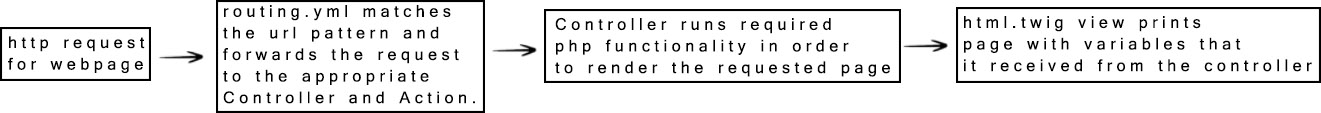
\includegraphics[scale=0.33]{symfonySystem.jpg}}
\caption{text text text text text}
\end{figure}
text text text text text text text text text text text text text text text\\text text text text text text text text text text text text text text text\\text text text text text text text text text text text text text text text\\text text text text text text text text text text text text text text text\\

\subsubsection{Refactoring}
text text text text text text text text text text text text text text text\\text text text text text text text text text text text text text text text\\text text text text text text text text text text text text text text text\\text text text text text text text text text text text text text text text\\text text text text text text text text text text text text text text text\\

\subsection*{Game}
\subsubsection{Design}
text text text text text text text text text text text text text text text\\text text text text text text text text text text text text text text text\\text text text text text text text text text text text text text text text\\
\begin{enumerate}
\item text text text text text text text text text text text text text text text\\
\item text text text text text text text text text text text text text text text\\
\item text text text text text text text text text text text text text text text\\
\begin{enumerate}
\item text text text text text text text text text text text text text text text\\
\begin{itemize}
\item text text text text text text text text text text text text text text text\\
\item text text text text text text text text text text text text text text text\\
\item text text text text text text text text text text text text text text text\\
\item text text text text text text text text text text text text text text text\\
\item text text text text text text text text text text text text text text text\\
\item text text text text text text text text text text text text text text text\\
\item text text text text text text text text text text text text text text text\\
\item text text text text text text text text text text text text text text text\\
\end{itemize}  
\item text text text text text text text text text text text text text text text\\
\item text text text text text text text text text text text text text text text\\
\item text text text text text text text text text text text text text text text\\
\begin{itemize}
\item text text text text text text text text text text text text text text text\\
\item text text text text text text text text text text text text text text text\\
\item text text text text text text text text text text text text text text text\\
\end{itemize}
\item text text text text text text text text text text text text text text text\\
\item text text text text text text text text text text text text text text text\\
\begin{itemize}
\item text text text text text text text text text text text text text text text\\
\item text text text text text text text text text text text text text text text\\
\item text text text text text text text text text text text text text text text\\
\item text text text text text text text text text text text text text text text\\
\item text text text text text text text text text text text text text text text\\
\item text text text text text text text text text text text text text text text\\
\end{itemize}
text text text text text text text text text text text text text text text\\

\begin{figure}[h]
\centering
\makebox[\textwidth]{ \includegraphics[scale=0.31]{userGuide.jpg}}
\caption{Visual representation of the game room, displaying many of the modules mentioned above.}
\end{figure}

\end{enumerate}
\item text text text text text text text text text text text text text text text\\
\item text text text text text text text text text text text text text text text\\
\begin{enumerate}
\item text text text text text text text text text text text text text text text\\
\item text text text text text text text text text text text text text text text\\
\item text text text text text text text text text text text text text text text\\
\end{enumerate}
\end{enumerate}
\subsubsection{Refactoring}
text text text text text text text text text text text text text text text\\text text text text text text text text text text text text text text text\\text text text text text text text text text text text text text text text\\
\subsubsection{Function Structure}
text text text text text text text text text text text text text text text\\
\begin{figure}[h]
\makebox[\textwidth]{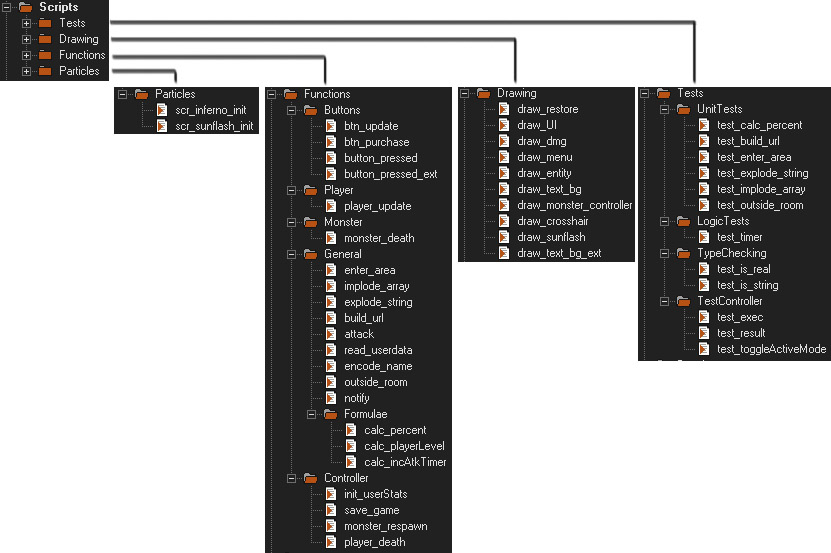
\includegraphics[scale=0.42]{script_hierachy.jpg}}
\caption{Script Hierachy, displaying the alignment of scripts used in gamemaker. Their content is located in the folder GM\_SOURCE/sourcecode/rendonan\_release.gmx/scripts.}
\end{figure}

\section*{Difficulties}
text text text text text text text text text text text text text text text\\text text text text text text text text text text text text text text text\\text text text text text text text text text text text text text text text\\
\begin{itemize}
\item text text text text text text text text text text text text text text text\\
\item text text text text text text text text text text text text text text text\\
\item text text text text text text text text text text text text text text text\\
\end{itemize}

\section*{Testing}
\subsection*{Website}
text text text text text text text text text text text text text text text\\text text text text text text text text text text text text text text text\\text text text text text text text text text text text text text text text\\text text text text text text text text text text text text text text text\\text text text text text text text text text text text text text text text\\
\begin{itemize}
\item text text text text text text text text text text text text text text text\\
\item text text text text text text text text text text text text text text text\\
\item text text text text text text text text text text text text text text text\\
\item text text text text text text text text text text text text text text text\\
\item text text text text text text text text text text text text text text text\\
\item text text text text text text text text text text text text text text text\\
\item text text text text text text text text text text text text text text text\\
\item text text text text text text text text text text text text text text text\\
\item text text text text text text text text text text text text text text text\\
\end{itemize}

\subsection*{Game}
text text text text text text text text text text text text text text text\\
\begin{enumerate}
\item \emph{\textbf{Type Checks:}} text text text text text text text text text text text text text text text\\
\item \emph{\textbf{Logic tests:}} text text text text text text text text text text text text text text text\\
\item \emph{\textbf{Unit tests:}} text text text text text text text text text text text text text text text\\
\item \emph{\textbf{Connection tests:}} text text text text text text text text text text text text text text text\\
\end{enumerate}
text text text text text text text text text text text text text text text\\text text text text text text text text text text text text text text text\\text text text text text text text text text text text text text text text\\
\subsection*{Test Coverage}
text text text text text text text text text text text text text text text\\text text text text text text text text text text text text text text text\\text text text text text text text text text text text text text text text\\

\section*{Deficiencies}
text text text text text text text text text text text text text text text\\text text text text text text text text text text text text text text text\\text text text text text text text text text text text text text text text\\
\begin{itemize}
\item text text text text text text text text text text text text text text text\\
\item text text text text text text text text text text text text text text text\\
\item text text text text text text text text text text text text text text text\\
\end{itemize}
text text text text text text text text text text text text text text text\\text text text text text text text text text text text text text text text\\text text text text text text text text text text text text text text text\\

\section*{Future Improvements}
\subsection*{Choice of technology / language}
text text text text text text text text text text text text text text text\\text text text text text text text text text text text text text text text\\text text text text text text text text text text text text text text text\\
\subsection*{Future project potentials}
text text text text text text text text text text text text text text text\\text text text text text text text text text text text text text text text\\text text text text text text text text text text text text text text text\\

\section*{Conclusion}
text text text text text text text text text text text text text text text\\
text text text text text text text text text text text text text text text\\
text text text text text text text text text text text text text text text\\

\end{document}
